\documentclass[a4paper]{article}

\usepackage[english]{babel}
\usepackage[utf8]{inputenc}
\usepackage{amsmath}
\usepackage{graphicx}
\usepackage[colorinlistoftodos]{todonotes}
\usepackage{caption}
\usepackage{subcaption}
\usepackage{here}

\title{Computational Photography}

\author{Mich\`ele Wyss, 10-104-123}

\date{December 11, 2014}

\graphicspath{{imgs/}}
\begin{document}
\maketitle

\section*{Ray space analysis}
\section*{EPI's}
Some example EPI's can be seen in Figure \ref{fig:EPIs}. 
The slopes of the lines vary with the depth of the object. 
For example, in the EPI of scanline 40, it's very well visible that the pink lines have a very different slope than all the other lines. 
This is because the pink animal is much closer to the camera than the rest and therefore seems to move faster when the camera drives by.
\begin{figure}[ht]
	\begin{subfigure}[h]{0.48\textwidth}
	  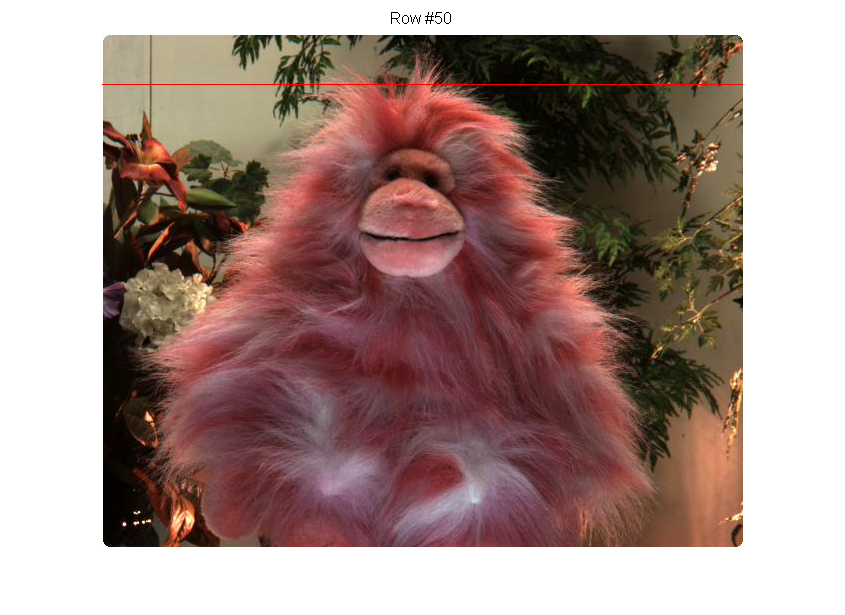
\includegraphics[width=\textwidth]{scanline50}
	  \caption*{Scanline at row 50}
	\end{subfigure}
    	~
	\begin{subfigure}[h]{0.48\textwidth}
	  \centering
	  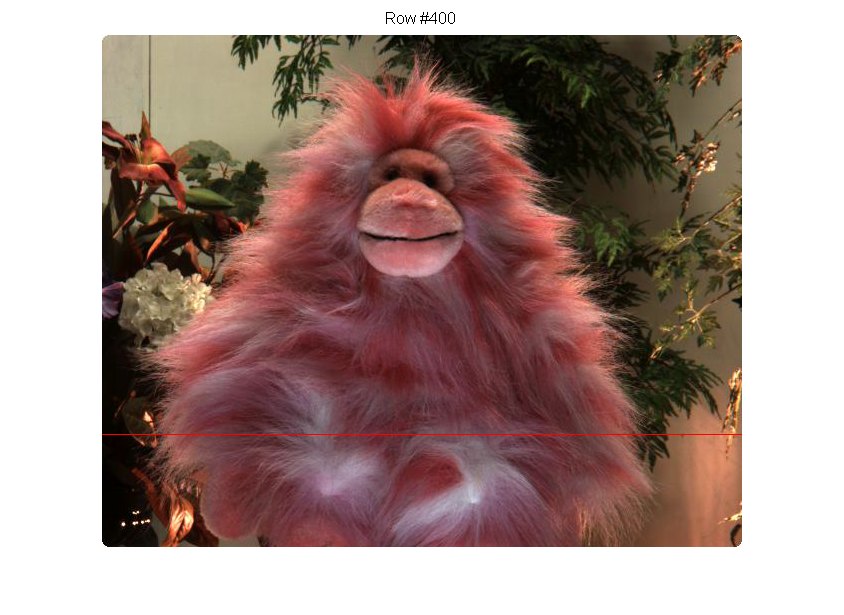
\includegraphics[width=\textwidth]{scanline400}
	  \caption*{Scanline at row 400}
	\end{subfigure}
	
	\vspace{3mm}
	\begin{subfigure}[h]{0.48\textwidth}
	  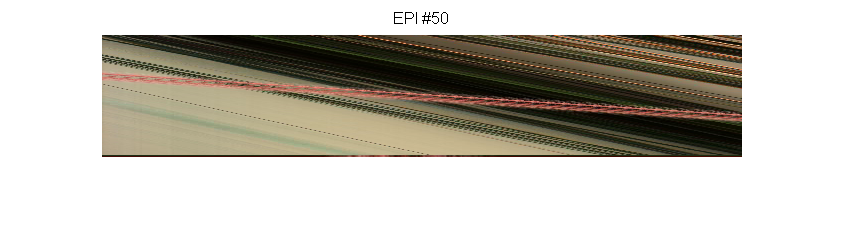
\includegraphics[width=\textwidth]{EPI50}
	  \caption*{EPI at 50}
	\end{subfigure}
    	~
	\begin{subfigure}[h]{0.48\textwidth}
	  \centering
	  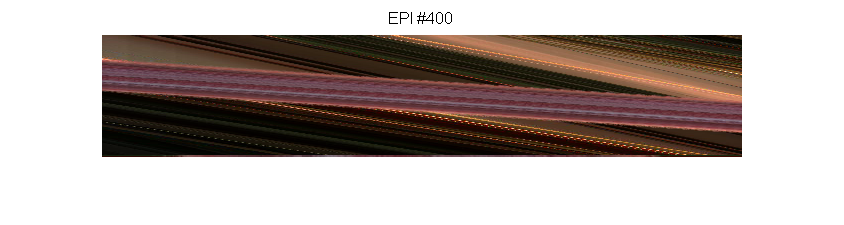
\includegraphics[width=\textwidth]{EPI400}
	  \caption*{EPI at row 400}
	\end{subfigure}
\caption{Examples of EPI's at two different scanlines of the pink animal scene.}
\label{fig:EPIs}
\end{figure}
\section*{Fourier Transform and visualized power spectrum}
In the Fourier transform, we can see the occuring frequencies. The slopes of the lines are perpendicular to the slopes of the lines in ray space. The horizontal is probably an artifact due to the borders.
\begin{figure}[ht]
	\vspace{2mm}
	\begin{subfigure}[h]{0.48\textwidth}
	  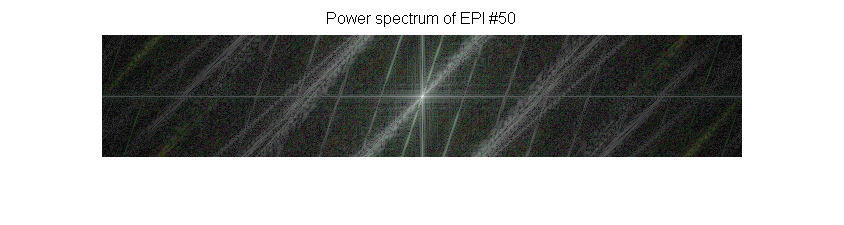
\includegraphics[width=\textwidth]{powerSpec50}
	  \caption*{Power spectrum at 50}
	\end{subfigure}
    	~
	\begin{subfigure}[h]{0.48\textwidth}
	  \centering
	  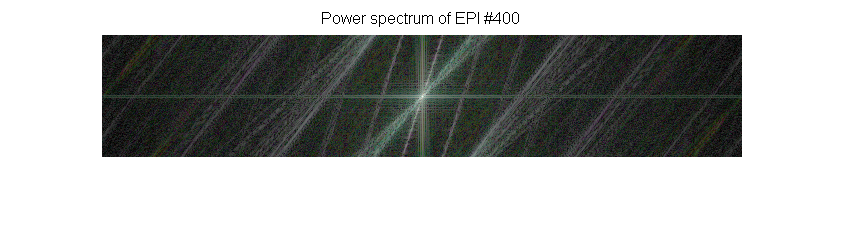
\includegraphics[width=\textwidth]{powerSpec400}
	  \caption*{Power spectrum at 400}
	\end{subfigure}
\caption{Visualized power spectrum of the two EPI's at scanlines 50 and 400.}
\label{fig:powerSpectrum}
\end{figure}

\section*{View Reconstruction}
\subsection*{Linear Interpolation}
Linearly interpolating two camera views results in double edges because the views are not aligned. With increasing $k$, the artifacts are more and more clearly visible (see for example Figure \ref{fig:linearInterpolation}). 
\begin{figure}[ht]
	\begin{subfigure}[h]{0.48\textwidth}
	  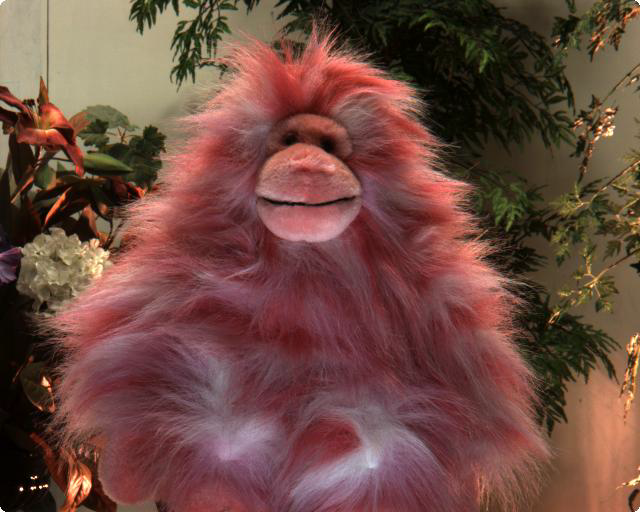
\includegraphics[width=\textwidth]{view60}
	  \caption*{View number 60}
	\end{subfigure}
    	~
	\begin{subfigure}[h]{0.48\textwidth}
	  \centering
	  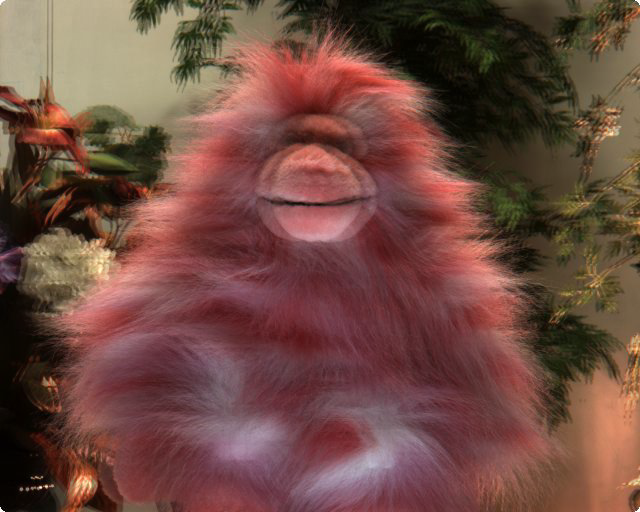
\includegraphics[width=\textwidth]{LinearInterpolation60_61}
	  \caption*{$k=1$}
	\end{subfigure}
	
	\vspace{2mm}
	\begin{subfigure}[h]{0.48\textwidth}
	  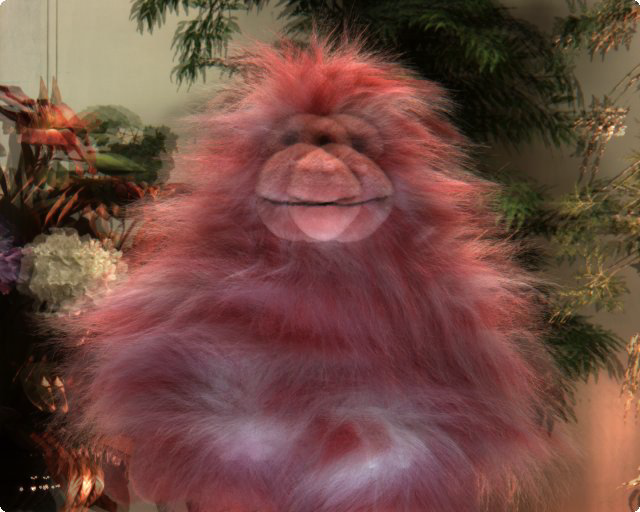
\includegraphics[width=\textwidth]{LinearInterpolation60_62}
	  \caption*{$k=2$}
	\end{subfigure}
    	~
	\begin{subfigure}[h]{0.48\textwidth}
	  \centering
	  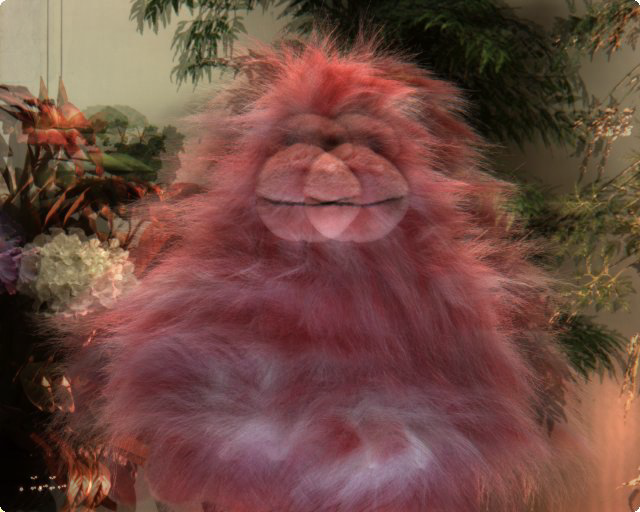
\includegraphics[width=\textwidth]{LinearInterpolation60_63}
	  \caption*{$k=3$}
	\end{subfigure}
	
	\vspace{2mm}
	\begin{subfigure}[h]{0.48\textwidth}
	  \centering
	  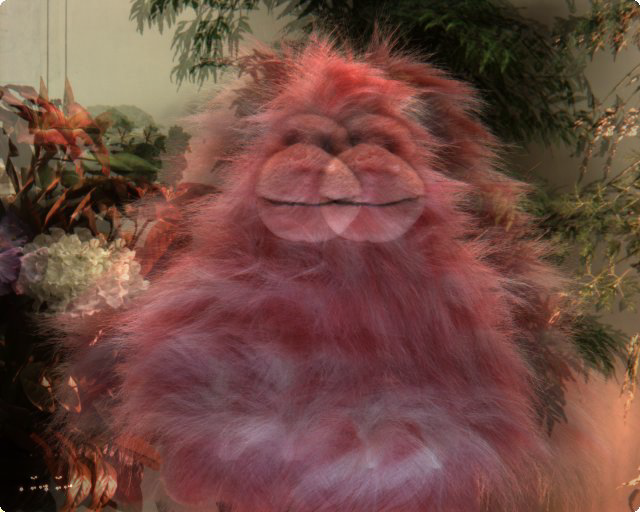
\includegraphics[width=\textwidth]{LinearInterpolation60_64}
	  \caption*{$k=4$}
	\end{subfigure}
	~
	\begin{subfigure}[h]{0.48\textwidth}
	  \centering
	  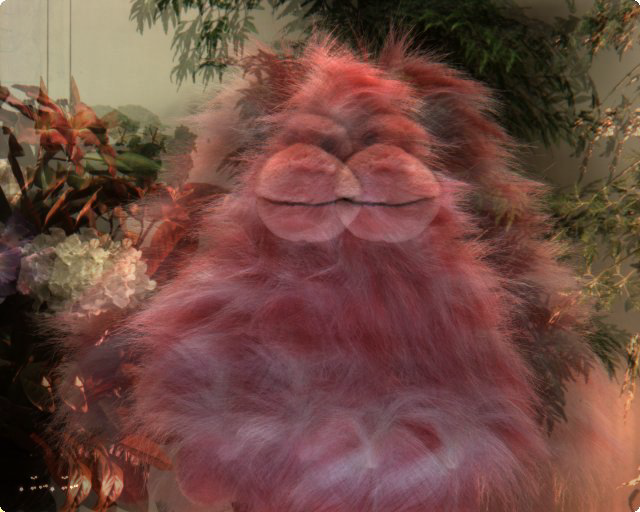
\includegraphics[width=\textwidth]{LinearInterpolation60_65}
	  \caption*{$k=5$}
	\end{subfigure}
\caption{Simple linear interpolation of the camera views $60$ and $(60 + k)$ in ray space leads to very large artifacts (double edges).}
\label{fig:linearInterpolation}
\end{figure}
\subsection*{Sheared Inpterpolation}
Using sheared interpolation, the results can be improved. The objects are aligned in depth by shearing the EPI's. The depth correspond to a slope in ray space. The depth in focus is the one depth where the slope is a vertical line in ray space. So, in order to focus on the pink animal, we want the pink lines to be vertical in the EPI's. In Figure \ref{fig:shearedInterpolationEPIs}, different shears of the EPI at scanline 70 can be seen. It seems that 16 pixels is the best we can get in order to make the pink line vertical.
\begin{figure}[ht]
	\begin{subfigure}[h]{0.48\textwidth}
	  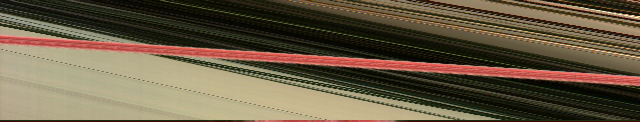
\includegraphics[width=\textwidth]{shear0}
	  \caption*{Original EPI \#70}
	\end{subfigure}
    	~
	\begin{subfigure}[h]{0.48\textwidth}
	  \centering
	  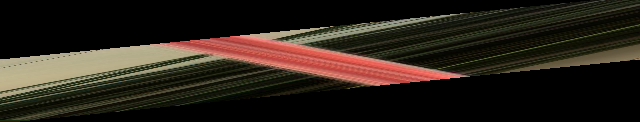
\includegraphics[width=\textwidth]{shear10}
	  \caption*{10 pixels shear}
	\end{subfigure}
	
	\vspace{2mm}
	\begin{subfigure}[h]{0.48\textwidth}
	  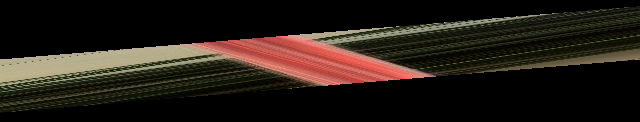
\includegraphics[width=\textwidth]{shear12}
	  \caption*{12 pixels shear}
	\end{subfigure}
    	~
	\begin{subfigure}[h]{0.48\textwidth}
	  \centering
	  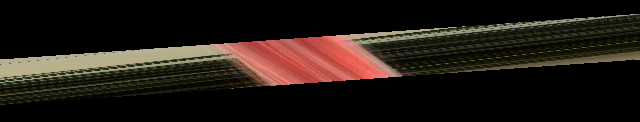
\includegraphics[width=\textwidth]{shear14}
	  \caption*{14 pixels shear}
	\end{subfigure}
	
	\vspace{2mm}
	\begin{subfigure}[h]{0.48\textwidth}
	  \centering
	  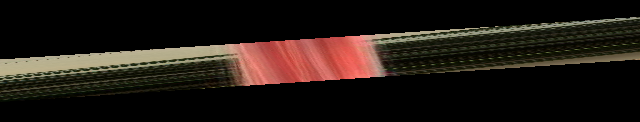
\includegraphics[width=\textwidth]{shear15}
	  \caption*{15 pixels shear}
	\end{subfigure}
	~
	\begin{subfigure}[h]{0.48\textwidth}
	  \centering
	  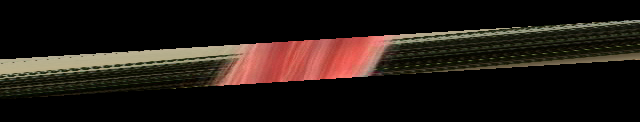
\includegraphics[width=\textwidth]{shear16}
	  \caption*{16 pixels shear}
	\end{subfigure}
		
	\vspace{2mm}
	\begin{subfigure}[h]{0.48\textwidth}
	  \centering
	  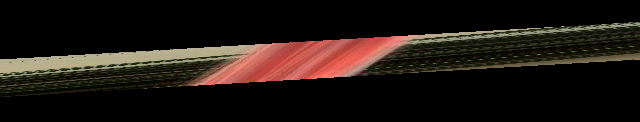
\includegraphics[width=\textwidth]{shear17}
	  \caption*{17 pixels shear}
	\end{subfigure}
	~
	\begin{subfigure}[h]{0.48\textwidth}
	  \centering
	  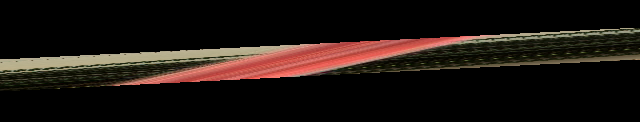
\includegraphics[width=\textwidth]{shear20}
	  \caption*{20 pixels shear}
	\end{subfigure}
\caption{The EPI at scanline 70, with different shears. Shearing by 16 pixels seems to yield the best result to make the pink line vertical.}
\label{fig:shearedInterpolationEPIs}
\end{figure}

Interpolating the sheared EPI's corresponds to a sheard interpolation and the results are clearly better than without the shear. See some results for different numbers of $k$ and a shear of 16 pixels in Figure \ref{fig:shearedInterpolationDifferentK}. Note that with increasing shear, the image size decreases because of the missing values caused by the translation of the single scanlines (dark boundaries on the left and right side of the images in Figures \ref{fig:shearedInterpolationDifferentK} and \ref{fig:shearedInterpolationDifferentShear}.
\begin{figure}[ht]
	\begin{subfigure}[h]{0.48\textwidth}
	  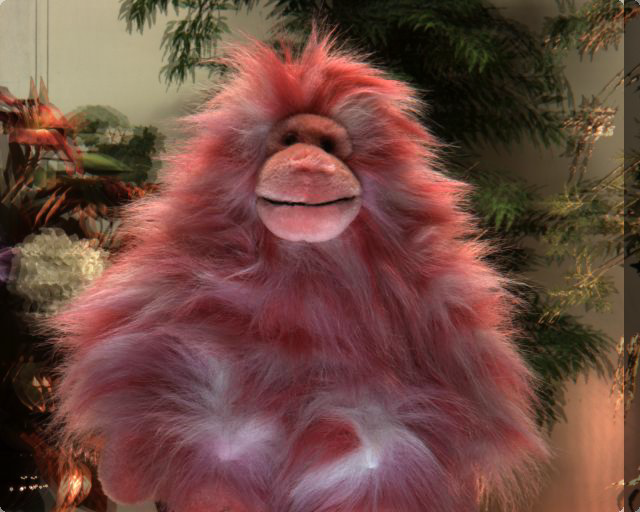
\includegraphics[width=\textwidth]{ShearedInterpolation60_61}
	  \caption*{$k = 1$}
	\end{subfigure}
    	~
	\begin{subfigure}[h]{0.48\textwidth}
	  \centering
	  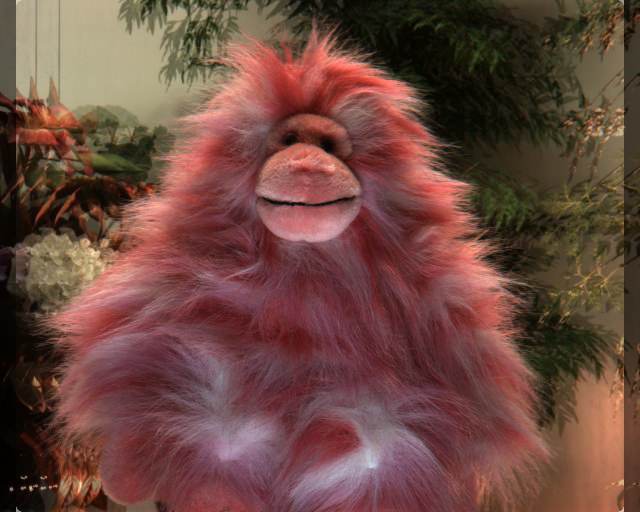
\includegraphics[width=\textwidth]{ShearedInterpolation59_61}
	  \caption*{$k= 2$}
	\end{subfigure}
	
	\vspace{2mm}
	\begin{subfigure}[h]{0.48\textwidth}
	  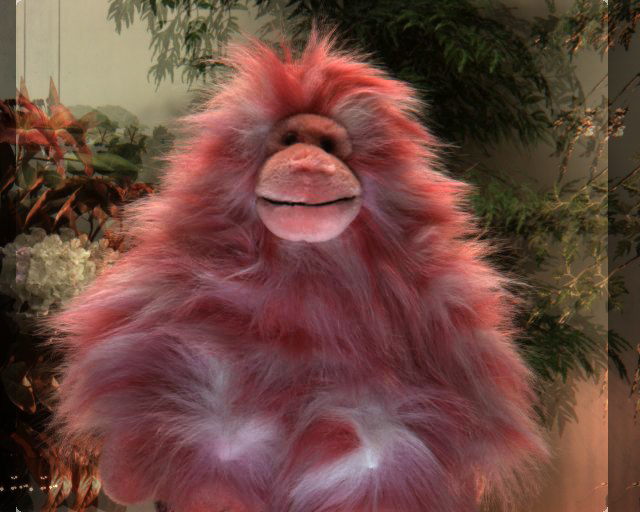
\includegraphics[width=\textwidth]{ShearedInterpolation59_62}
	  \caption*{$k=3$}
	\end{subfigure}
    	~
	\begin{subfigure}[h]{0.48\textwidth}
	  \centering
	  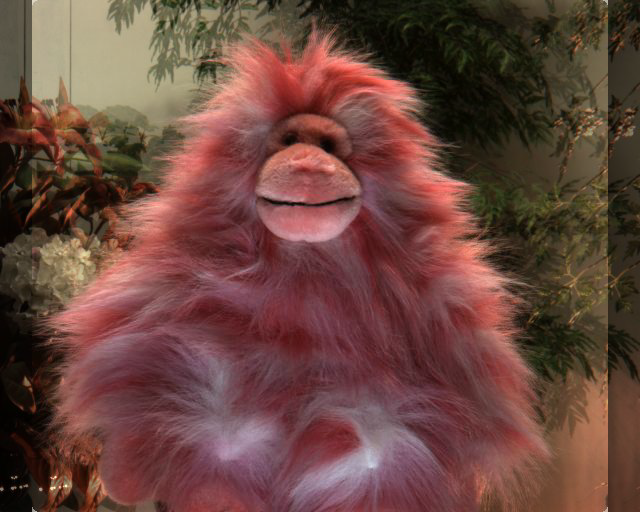
\includegraphics[width=\textwidth]{ShearedInterpolation58_62}
	  \caption*{$k=4$}
	\end{subfigure}
	
	\vspace{2mm}
	\begin{subfigure}[h]{0.48\textwidth}
	  \centering
	  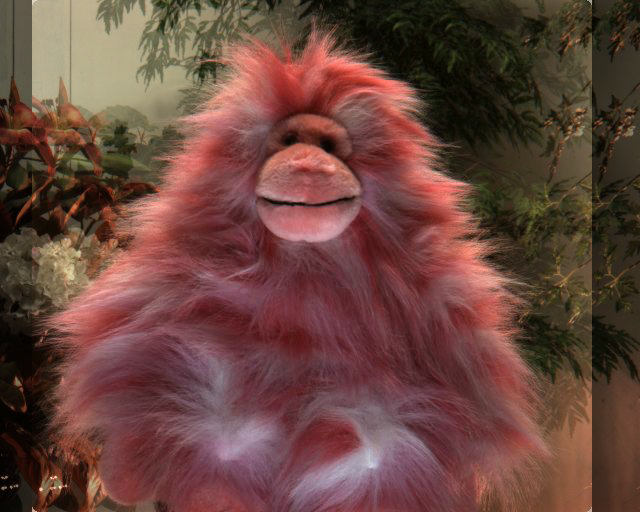
\includegraphics[width=\textwidth]{ShearedInterpolation58_63}
	  \caption*{$k=5$}
	\end{subfigure}
	~
	\begin{subfigure}[h]{0.48\textwidth}
	  \centering
	  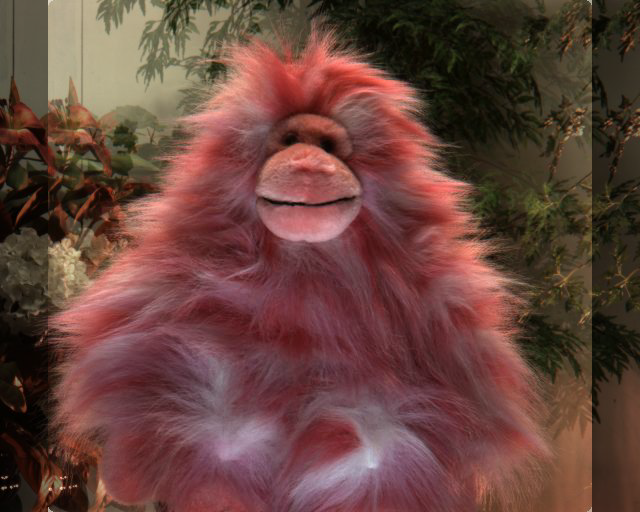
\includegraphics[width=\textwidth]{ShearedInterpolation57_63}
	  \caption*{k=6}
	\end{subfigure}
\caption{Some results obtained by interpolating the sheared EPI's using a shear of 16 pixels.}
\label{fig:shearedInterpolationDifferentK}
\end{figure}
For some examples of what happens with different shears, see Figure \ref{fig:shearedInterpolationDifferentShear}. Different shears cause other depths to be in focus, namely the ones that are vertical in the sheared EPI. Especially, some shears can cause very bad results if the corresponding vertical line does not appear in the EPI, that is, when there's no object at a particular depth in the scene. This leads to an image where everything is out of focus.
\begin{figure}[ht]
	\begin{subfigure}[h]{0.48\textwidth}
	  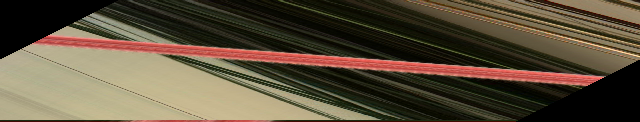
\includegraphics[width=\textwidth]{shear2}
	  
	  \vspace{2mm}
	  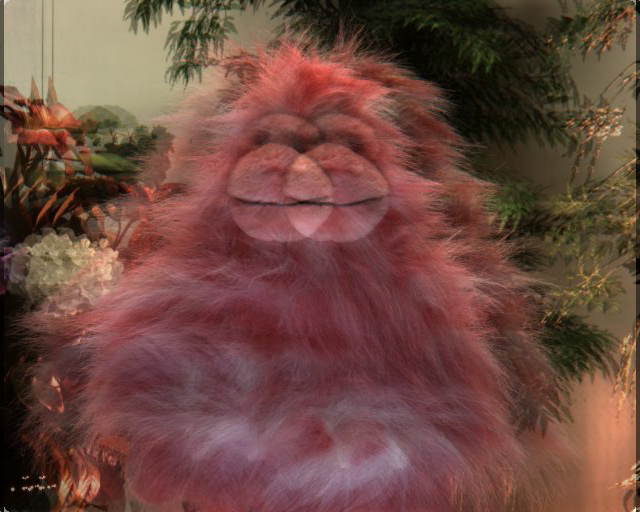
\includegraphics[width=\textwidth]{ShearedInterpolation58_62_shear2}
	  \caption*{2 pixels shear}
	\end{subfigure}
    	~
	\begin{subfigure}[h]{0.48\textwidth}
	  \centering
	  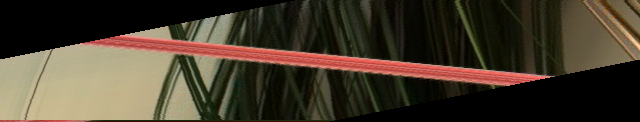
\includegraphics[width=\textwidth]{shear5}
	  
	  \vspace{2mm}
	  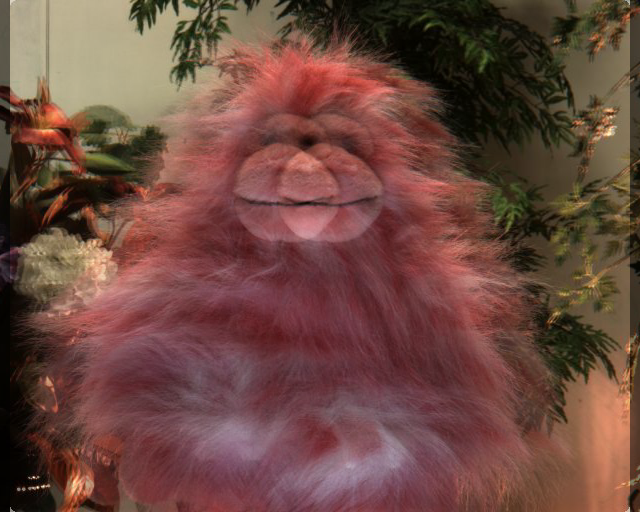
\includegraphics[width=\textwidth]{ShearedInterpolation58_62_shear5}
	  \caption*{5 pixels shear}
	\end{subfigure}
	
	\vspace{2mm}
	\begin{subfigure}[h]{0.48\textwidth}
	  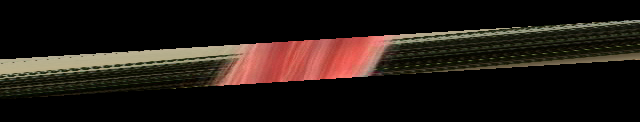
\includegraphics[width=\textwidth]{shear16}
	  
	  \vspace{2mm}
	  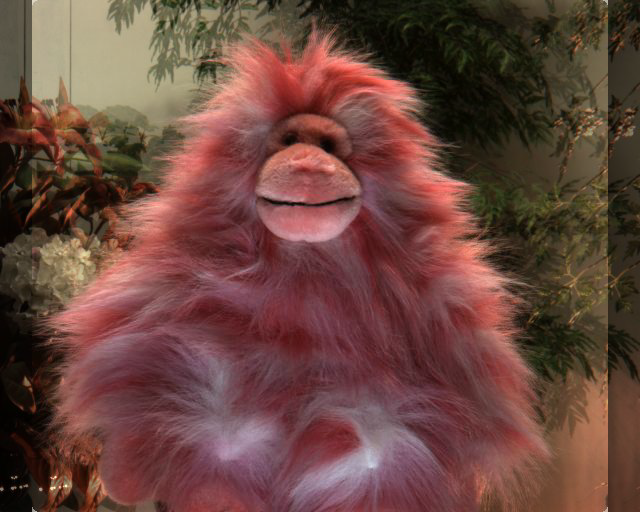
\includegraphics[width=\textwidth]{ShearedInterpolation58_62_shear16}
	  \caption*{16 pixels shear}
	\end{subfigure}
    	~
	\begin{subfigure}[h]{0.48\textwidth}
	  \centering
	  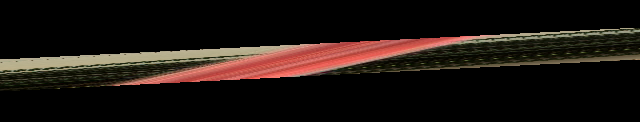
\includegraphics[width=\textwidth]{shear20}
	  
	  \vspace{2mm}
	  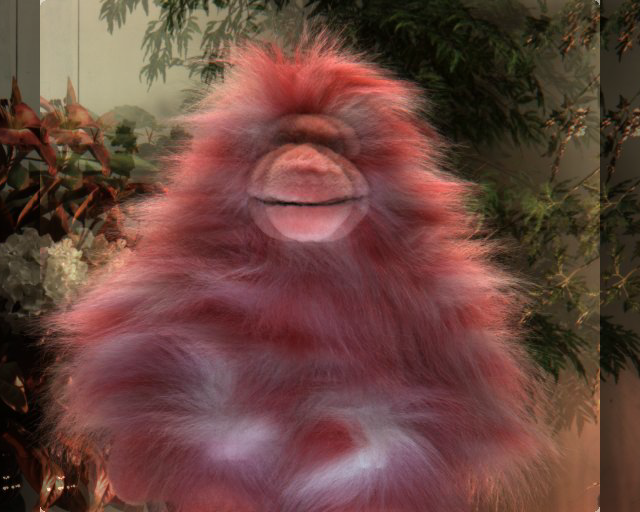
\includegraphics[width=\textwidth]{ShearedInterpolation58_62_shear20}
	  \caption*{20 pixels shear}
	\end{subfigure}
\caption{Some results obtained by different amounts of shear and a value of $k=4$. Note that e.g.\ with the 5 pixels shear, there are some things from the background in focus, whereas the 16 pixels shear is focused on the pink animal. The other shears don't focus any of the appearing depths in the image which can be seen from the visualized EPI's. (no vertical lines)}
\label{fig:shearedInterpolationDifferentShear}
\end{figure}

\subsection*{Filtering with Gaussian kernel}
Filtering the sheared EPI's with Gaussian kernels before interpolating them yield out-of-focus blurs (instead of doubled edges) for the scene depths that are not in focus. Some examples can be seen in Figures \ref{fig:shearedInterpolationGaussDifferentShear} 

\begin{figure}[ht]
	\begin{subfigure}[h]{0.48\textwidth}
	  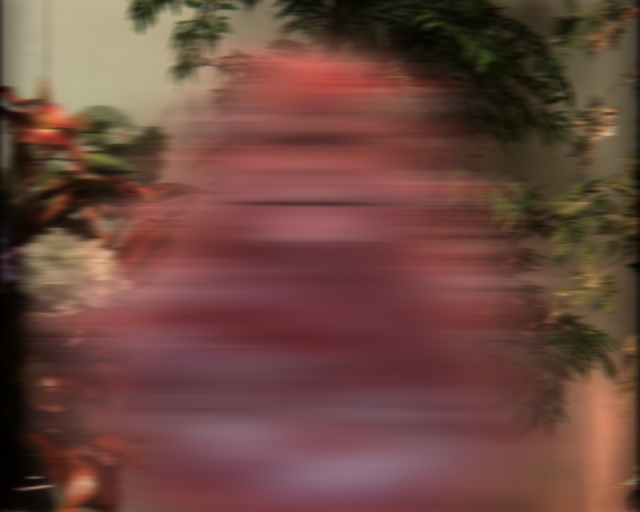
\includegraphics[width=\textwidth]{shearedGauss_k1_shear5_sighor4_sigvert5}
	  \caption*{Background in focus \\(shear = 5)}
	\end{subfigure}
    	~
	\begin{subfigure}[h]{0.48\textwidth}
	  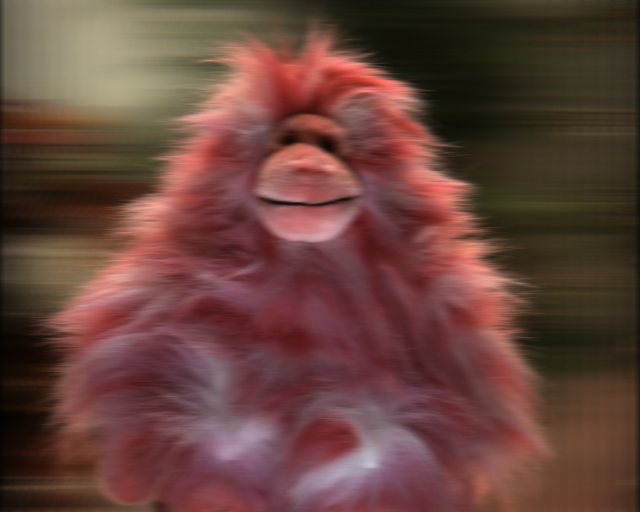
\includegraphics[width=\textwidth]{shearedGauss_k1_shear16_sighor4_sigvert5}
	  \caption*{Animal in focus \\(shear = 16)}
	\end{subfigure}
\caption{Two images with different shears. The EPI's were blurred using a Gaussian elliptical filter with $\sigma_{horizontal} = 4$ and $\sigma_{vertical} = 5$. The two inteprolated views are consecutive, i.e.\ $k=1$.}
\label{fig:shearedInterpolationGaussDifferentShear}
\end{figure}

\begin{figure}[ht]
	\begin{subfigure}[h]{0.48\textwidth}
	  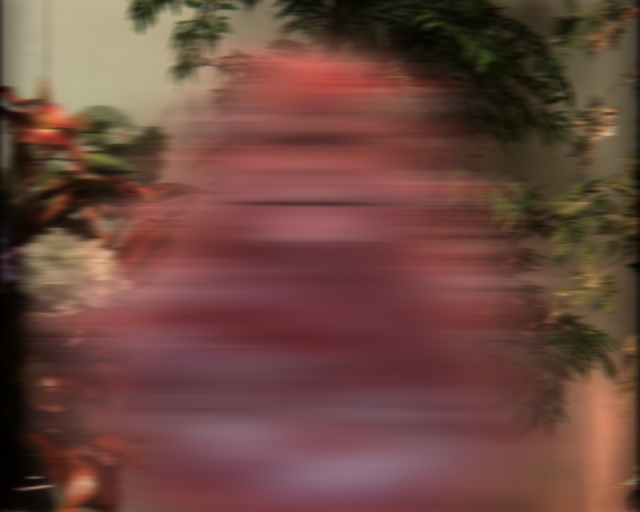
\includegraphics[width=\textwidth]{shearedGauss_k1_shear5_sighor4_sigvert5}
	  \caption*{Background in focus \\(shear = 5)}
	\end{subfigure}
    	~
	\begin{subfigure}[h]{0.48\textwidth}
	  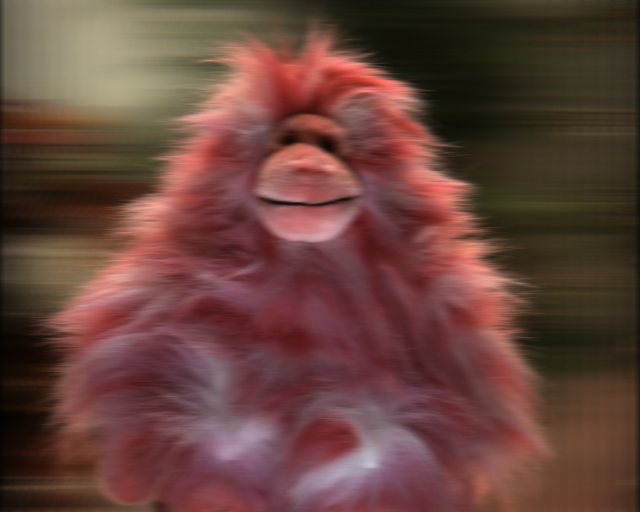
\includegraphics[width=\textwidth]{shearedGauss_k1_shear16_sighor4_sigvert5}
	  \caption*{Animal in focus \\(shear = 16)}
	\end{subfigure}
\caption{The same example as in Figure \ref{fig:shearedInterpolationGaussDifferentShear}, but with $k=4$.}
\label{fig:shearedInterpolationGaussDifferentK}
\end{figure}

The filter size of the Gaussian filter determines the depth of field. A small filter size corresponds to a small synthetic aperture (large depth of field), and vice versa. Some examples of different filter sizes can be seen in Figures \ref{fig:shearedInterpolationGaussDifferentFilterSize1}, \ref{fig:shearedInterpolationGaussDifferentFilterSize2} and \ref{fig:shearedInterpolationGaussDifferentFilterSize3}. If we adapt the shear such that the background is in focus and use a large enough synthetic aperture size, we can theoretically ``see through'' the foreground object (see Figure \ref{fig:seeThrough}).
\begin{figure}[ht]
	\begin{subfigure}[h]{0.48\textwidth}
	  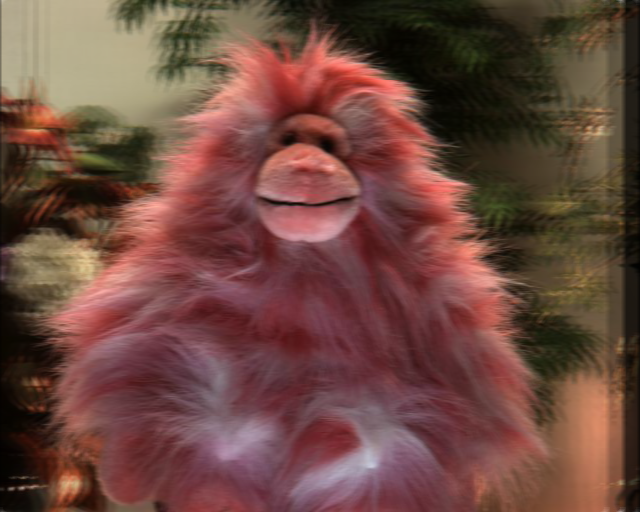
\includegraphics[width=\textwidth]{shearedGauss_k1_shear16_sighor2_sigvert0-5}
	  \caption*{$\sigma_{horizontal} = 2, \sigma_{vertical} = 0.5$}
	\end{subfigure}
    	~
	\begin{subfigure}[h]{0.48\textwidth}
	  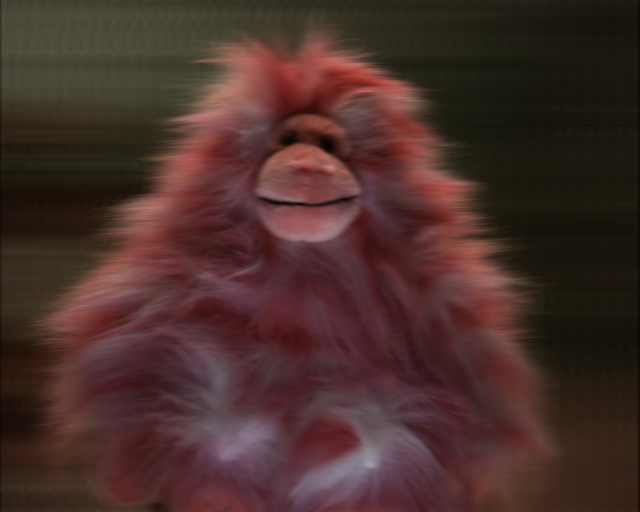
\includegraphics[width=\textwidth]{shearedGauss_k1_shear16_sighor2_sigvert20}
	  \caption*{$\sigma_{horizontal} = 2, \sigma_{vertical} = 20$}
	\end{subfigure}
	
	\vspace{2mm}
	\begin{subfigure}[h]{0.48\textwidth}
	  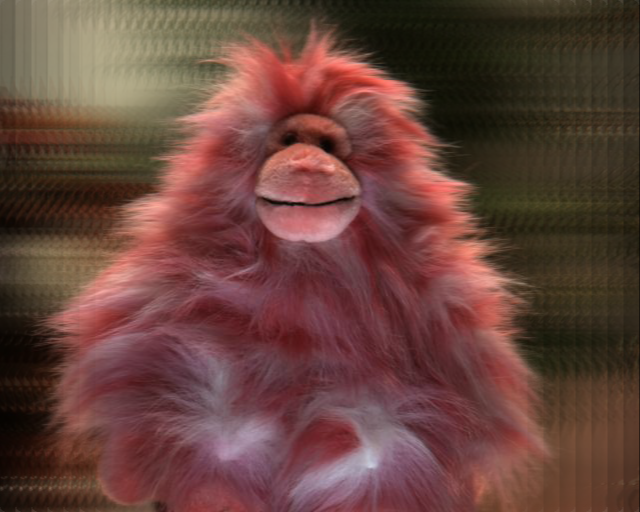
\includegraphics[width=\textwidth]{shearedGauss_k1_shear16_sighor0-5_sigvert5}
	  \caption*{$\sigma_{horizontal} = 0.5, \sigma_{vertical} = 5$}
	\end{subfigure}
    	~
	\begin{subfigure}[h]{0.48\textwidth}
	  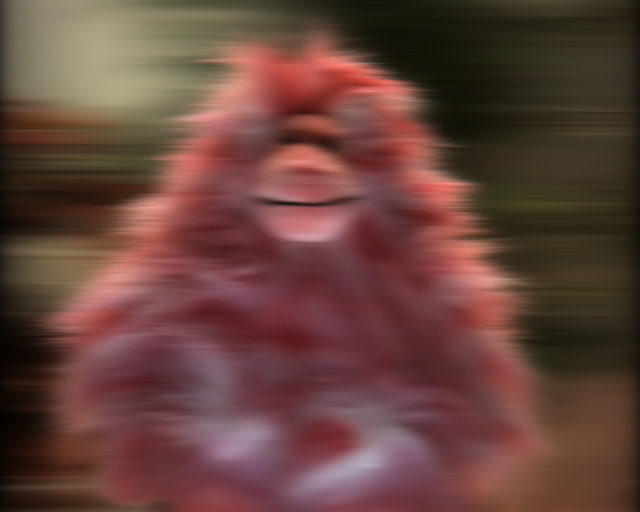
\includegraphics[width=\textwidth]{shearedGauss_k1_shear16_sighor20_sigvert5}
	  \caption*{$\sigma_{horizontal} = 20, \sigma_{vertical} = 5$}
	\end{subfigure}
\caption{The same example as in Figure \ref{fig:shearedInterpolationGaussDifferentShear}, but with $k=4$.}
\label{fig:shearedInterpolationGaussDifferentFilterSize1}
\end{figure}

\begin{figure}[ht]
	\begin{subfigure}[h]{0.48\textwidth}
	  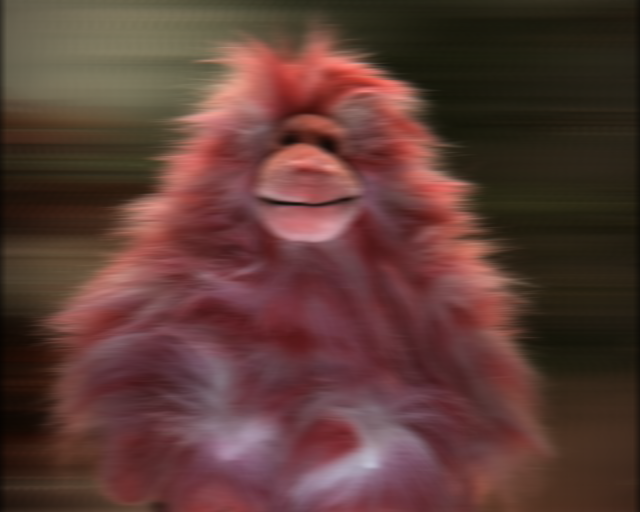
\includegraphics[width=\textwidth]{shearedGauss_k1_shear16_sighor5_sigvert10}
	  \caption*{$\sigma_{horizontal} = 5, \sigma_{vertical} = 10$}
	\end{subfigure}
    	~
	\begin{subfigure}[h]{0.48\textwidth}
	  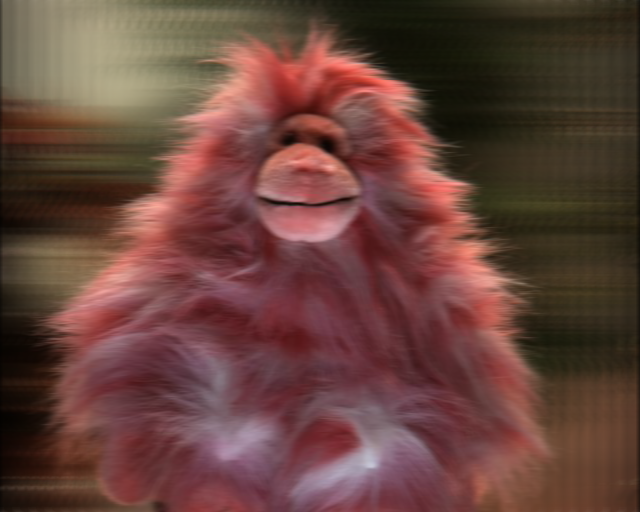
\includegraphics[width=\textwidth]{shearedGauss_k1_shear16_sighor2-5_sigvert5}
	  \caption*{$\sigma_{horizontal} = 2.5, \sigma_{vertical} = 5$}
	\end{subfigure}
	
	\vspace{2mm}
	\begin{subfigure}[h]{0.48\textwidth}
	  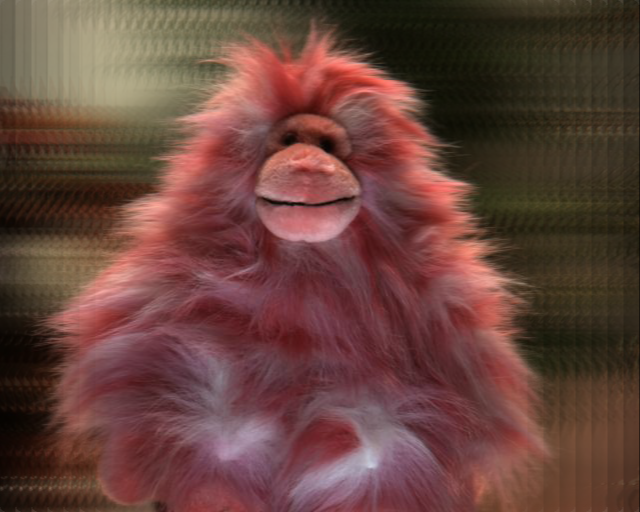
\includegraphics[width=\textwidth]{shearedGauss_k1_shear16_sighor0-5_sigvert5}
	  \caption*{$\sigma_{horizontal} = 0.5, \sigma_{vertical} = 5$}
	\end{subfigure}
    	~
	\begin{subfigure}[h]{0.48\textwidth}
	  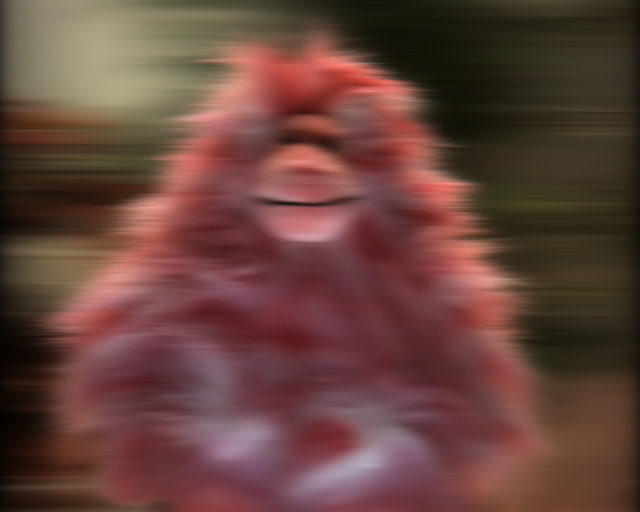
\includegraphics[width=\textwidth]{shearedGauss_k1_shear16_sighor20_sigvert5}
	  \caption*{$\sigma_{horizontal} = 20, \sigma_{vertical} = 5$}
	\end{subfigure}
\caption{The same example as in Figure \ref{fig:shearedInterpolationGaussDifferentShear}, but with $k=4$.}
\label{fig:shearedInterpolationGaussDifferentFilterSize2}
\end{figure}

\begin{figure}[ht]
	\begin{subfigure}[h]{0.48\textwidth}
	  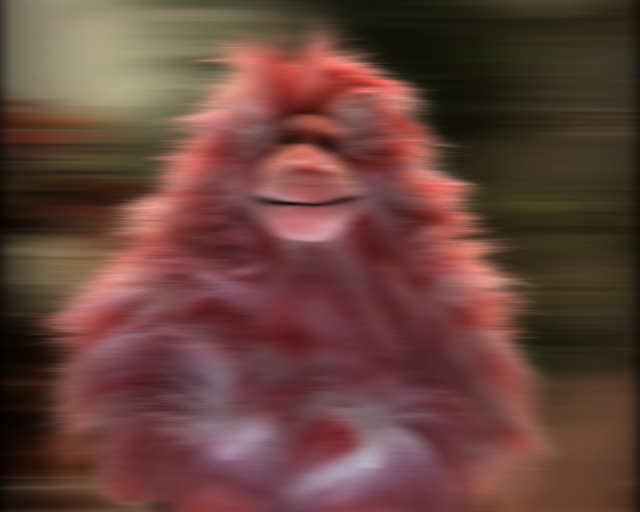
\includegraphics[width=\textwidth]{shearedGauss_k1_shear16_sighor10_sigvert5}
	  \caption*{$\sigma_{horizontal} = 10, \sigma_{vertical} = 5$}
	\end{subfigure}
    	~
	\begin{subfigure}[h]{0.48\textwidth}
	  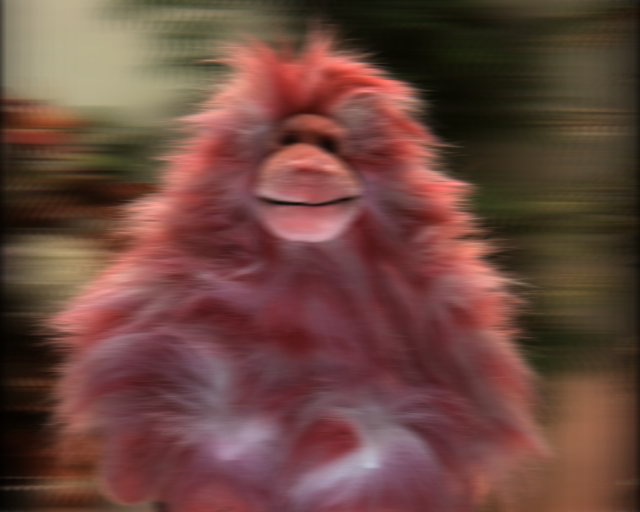
\includegraphics[width=\textwidth]{shearedGauss_k1_shear16_sighor5_sigvert2-5}
	  \caption*{$\sigma_{horizontal} = 5, \sigma_{vertical} = 2.5$}
	\end{subfigure}
	
	\vspace{2mm}
	\begin{subfigure}[h]{0.48\textwidth}
	  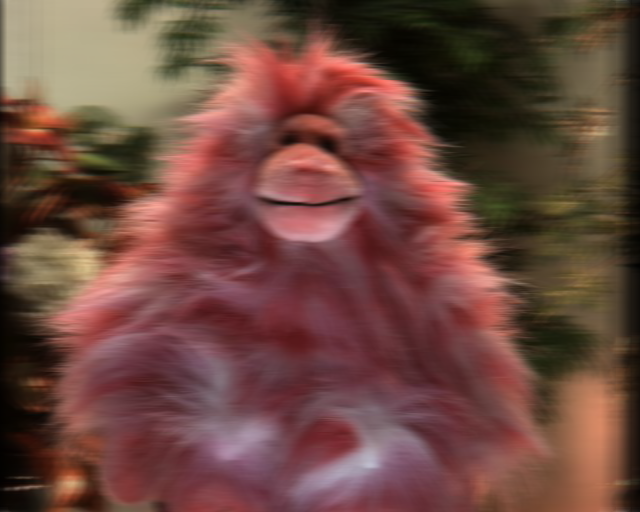
\includegraphics[width=\textwidth]{shearedGauss_k1_shear16_sighor5_sigvert0-5}
	  \caption*{$\sigma_{horizontal} = 5, \sigma_{vertical} = 0.5$}
	\end{subfigure}
    	~
	\begin{subfigure}[h]{0.48\textwidth}
	  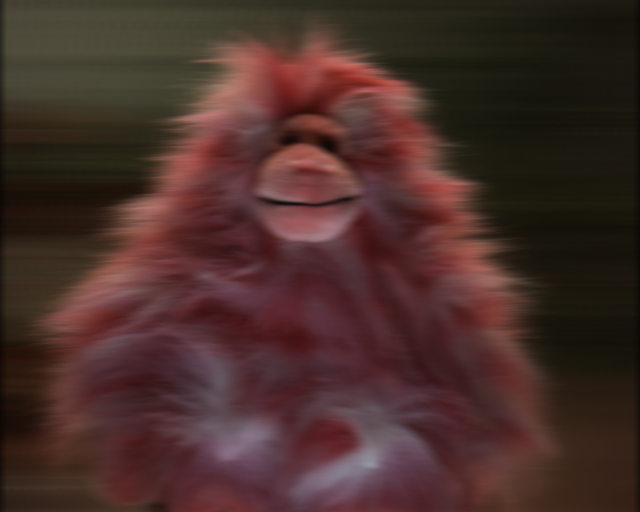
\includegraphics[width=\textwidth]{shearedGauss_k1_shear16_sighor5_sigvert20}
	  \caption*{$\sigma_{horizontal} = 5, \sigma_{vertical} = 20$}
	\end{subfigure}
\caption{The same example as in Figure \ref{fig:shearedInterpolationGaussDifferentShear}, but with $k=4$.}
\label{fig:shearedInterpolationGaussDifferentFilterSize3}
\end{figure}

\begin{figure}[ht]
	\begin{subfigure}[h]{0.48\textwidth}
	  \includegraphics[width=\textwidth]{shearedGauss_k20_shear5_sighor10_sigvert30}
	  \caption*{$k=4,\sigma_{horizontal} = 10, \sigma_{vertical} = 30$}
	\end{subfigure}
    	~
	\begin{subfigure}[h]{0.48\textwidth}
	  \includegraphics[width=\textwidth]{shearedGauss_k5_shear5_sighor5_sigvert45}
	  \caption*{$k=5, \sigma_{horizontal} = 5, \sigma_{vertical} = 45$}
	\end{subfigure}
\caption{Using a large filter size, we can simulate a large synthetic aperture and see through some objects.}
\label{fig:seeThrough}
\end{figure}
\end{document}